\documentclass[10pt]{beamer}

\usepackage[english]{babel}
\usepackage[utf8]{inputenc}
\usepackage{amsmath}
\usepackage{amssymb}
\usepackage{amsthm}
\usepackage[all]{xy}
\usepackage{graphicx}
\usepackage[style=beamer,doi=false,isbn=false,eprint=false,maxnames=10]{biblatex}
\bibliography{defeo}
\usepackage{mysymbols}

\usepackage[amssymb,amsfonts]{concmath}
\renewcommand{\sfdefault}{uop}
\mode<presentation>{%
  \usetheme{Boadilla}
  \usefonttheme[onlymath]{serif}
  \usecolortheme[rgb={0.56,0.3,0}]{structure}
  \setbeamercolor{alerted text}{fg=blue}
}
\renewcommand{\emph}[1]{{\usebeamercolor[fg]{structure}#1}}

\title[Explicit isogenies]{Explicit isogenies: recent progress and implementations}
\author{Luca~De~Feo}
\institute[IRMAR]{IRMAR, Université de Rennes 1}
\date[C2, April 4, 2011]{April 4, 2011\\C2, CAES CNRS, Saint-Pierre d'Oléron}


\begin{document}

\begin{frame}
  \titlepage
\end{frame}

%%

\begin{frame}
  \frametitle{Elliptic curves}

  \begin{itemize}
  \item Curves of genus $1$,
  \item Abelian varieties of dimension $1$.
  \end{itemize}
  
  \begin{block}{(Short) Weierstrass form}
    Assuming $p\ne2,3$
    {\large
      \begin{equation*}
        E\;:\;y^2 = x^3 + ax + b\qquad\text{with $a,b\in\K$.}
      \end{equation*}
    }
    \begin{itemize}
    \item discriminant: \alert{$\Delta_E = -16(4a^3 + 27b^2) \ne 0$} (the curve is non-singular),
    \item $j$-invariant: \alert{$j_E=\frac{-1728(4a^3)}{\Delta_E}$}
      ($j_E=j_{E'} \Leftrightarrow E\isom E'$ over $\clot{K}$),
    \item invariant differential: \alert{$\omega_E= \diff x/(2y)$} (invariant under translation).
    \end{itemize}
  \end{block}
\end{frame}

%%

%%

\begin{frame}
  \frametitle{Group law and scalar multiplication}
  
  \begin{columns}
    \begin{column}{0.3\textwidth}
      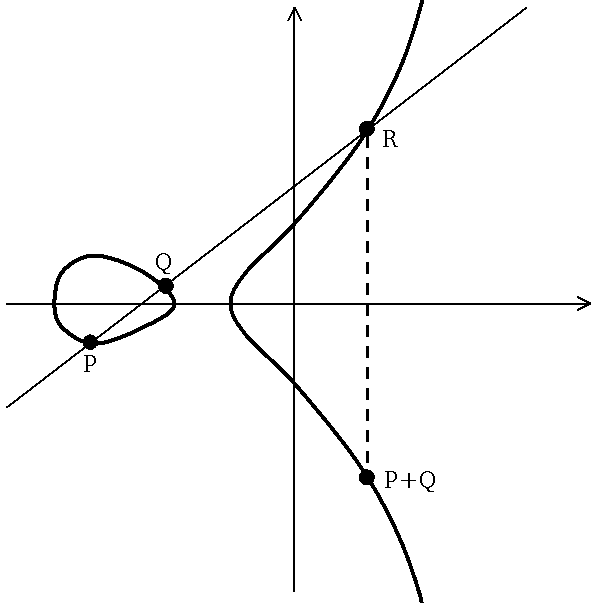
\includegraphics[width=\textwidth]{ecadd.png}
    \end{column}
    \begin{column}{0.55\textwidth}
      {\large\emph{\[y^2 = x^3 + ax + b\]}}
      \begin{gather*}
        P = (x_0, y_0), Q = (x_1, y_1)\\
        \lambda = \frac{y_1 - y_0}{x_1 - x_0}\\
        P+Q = (\lambda^2 - x_0 - x_1, (x_0 - x_2)\lambda - y_0)
      \end{gather*}
    \end{column}
  \end{columns}

  {\large
    \begin{description}
    \item[\emph{Multiplication:}] $[m]P = \overbrace{P + P + \cdots + P}^{\text{$m$ times}}$
    \item[\emph{$m$-torsion:}] $E[m] = \{P\in E(\clot{\K}) | [m]P=\0\} \isom (\Z/m\Z)^2$
    \end{description}}
  
  \[[m](x,y) = \left(\frac{\psi_m(x,y)}{\phi_m^2(x,y)}, \frac{\omega_m(x,y)}{\phi_m^3(x,y)}\right)\]
  
  \emph{Division polynomials:} $\phi_m$ can be computed with $O(\log
  m)$ polynomial multiplications, $\deg\phi_m=O(m^2)$.
\end{frame}

%%

% \begin{frame}
%   \frametitle{Elliptic curves over $\C$}

%   \begin{center}
%     Nice picture goes here
%   \end{center}
  
%   \begin{block}{Weierstrass $\wp$-function}
%     \[\wp(z) = \frac{1}{z^2} +
%     \sum_{\omega\in\Lambda\backslash\{0\}}\frac{1}{(z-\omega)^2}-\frac{1}{\omega^2}\]

%     Satisfies
%     \begin{equation*}
%       {\wp'}^2 = 4\wp^3 - 60G_4\wp - 140G_6.
%     \end{equation*}

%     We have an isomorphism:
%     \begin{equation*}
%       \begin{aligned}
%         \C/\Lambda &\to E(\C)\\
%         z &\mapsto\left(\wp(z),\wp'(z)\right).
%       \end{aligned}
%     \end{equation*}
%   \end{block}
% \end{frame}

%%

\begin{frame}
  \frametitle{Isogenies}
  
  \vspace{-5mm}

  {\large \[\xymatrix{E\ar[d]_{[m]}\ar[r]^{\I} & E'\ar[dl]^{\hat{\I}}\\E}\]} 
  \emph{\textbf{(Separable) isogeny:}} (separable)
  non-constant rational morphism preserving the identity.
  
  \begin{block}{Properties}
    \begin{itemize}
    \item Isogeny = rational map $\;+\;$ group morphism;
    \item Finite kernel, surjective (in $\clot{\K}$);
    \item \emph{Dual isogeny theorem:} they factor the multiplication map into two pieces.
    \end{itemize}
  \end{block}

  \vspace{-1mm}

  \begin{block}{
	\begin{overprint}
	\onslide<1> Multiplication	
	\onslide<2> Frobenius endomorphism
	\onslide<3> Separable isogeny (short Weierstrass form)
	\end{overprint}
      }
    \begin{overprint}
      \onslide<1>
      \[\begin{aligned}
	{}[m] : E(\clot{\K}) &\rightarrow E(\clot{\K})\\
	                   P &\mapsto [m]P
      \end{aligned}\]
      $\ker\I = E[m]$.

      \onslide<2>
      \[\begin{aligned}
	\frob : E(\clot{\K}) &\rightarrow E(\clot{\K})\\
	               (x,y) &\mapsto (x^q,y^q)
      \end{aligned}\]
      $\ker\frob = \{\0\}$ (inseparable).

      \onslide<3>
      \[\quad\I(x,y) = \left(\frac{g(x)}{h(x)},
      cy\left(\frac{g(x)}{h(x)}\right)'\right)\]
      $h\;$ vanishes on the abscissas of $\;\ker\I$. \emph{$\quad\deg\I \;=\; \card{\ker\I}$}.
    \end{overprint}
  \end{block}  
\end{frame}

%%

\begin{frame}
  \frametitle{Why compute (large) isogenies over finite fields?}
  
  \begin{block}{SEA algorithm (\cite{schoof85,elkies92,atkin88})}
    \begin{description}
    \item[Hasse bound] \hfill{\large\emph{$\card{E(\F_q)}= q-t+1$}};\hfill\strut
    \item[Schoof] Compute $t$ modulo small primes
      $\ell\;\Leftrightarrow$ compute the action of $\frob_q$ on
      \emph{$E[\ell]\;\isom\;(\Z/\ell\Z)^2$};
    \item[Atkin] Determine the order of the roots of $X^2 -tX +q$ by
      factoring the $\ell$-th modular polynomial;
    \item[Elkies] Compute an $\ell$-isogeny $\I$ and the action of
      $\frob_q$ on \emph{$\ker\I\;\isom\;\Z/\ell\Z\;\subset\;E[\ell]$}.
    \end{description}
  \end{block}

  \begin{block}{Other cryptographic applications}
    \begin{itemize}
    \item Transfer DLPs between curves (\cite{gaudry+hess+smart02,smith09});
    \item Construct new cryptosystems (\cite{teske06,rostovtsev+stolbunov06});
    \item Construct hash functions (\cite{charles+lauter+goren09});
    \item Compute modular polynomials (\cite{sutherland10:modpol});
    \item Compute the endomorphism ring (\cite{kohel,bisson+sutherland11}).
    \end{itemize}
  \end{block}
\end{frame}

%%

\begin{frame}
  \frametitle{Vélu's formulas}
  
  \begin{block}{Compute an isogeny with given kernel (\cite{velu71})}
    Given the kernel $H$, computes $\;\I : E\to E/H\;$ given by
    \begin{align*}
      &\I(\0_E) = \I(\0_{E/H})\text{,}\\
      &\begin{aligned}
        \I(P) = \Biggl(x(P) + \sum_{Q\in H^\ast}x(P+Q) - x(Q),
        y(P) + \sum_{Q\in H^\ast}y(P+Q) - y(Q) \Biggr) \text{.}
      \end{aligned}
    \end{align*}
  \end{block}

  \begin{block}{In practice, given $h(x)$, of degree $\ell-1$,
      vanishing on $H$}
    {\footnotesize
      \[
      y^2 = f(x)\text{,}
      \qquad
      p_1 = \sum_{Q\in H^\ast} x(Q)\text{,}
      \qquad
      \frac{g(x)}{h(x)} = \ell x - p_1 - f'(x)\frac{h'(x)}{h(x)} - 2f(x)\left(\frac{h'(x)}{h(x)}\right)'\]}
    \[\alert{\I(x,y) = \left(\frac{g(x)}{h(x)}, y\left(\frac{g(x)}{h(x)}\right)'\right)}\]
  \end{block}
\end{frame}

%%


\begin{frame}
  \frametitle{Modular polynomial}

  \begin{center}
    $\Phi_\ell(X,Y)$, the minimal polynomial over $\C$ of the modular
    function $j(\ell\tau)$
  \end{center}

  \begin{block}{Properties}
    \begin{itemize}
    \item The roots of $\Phi_\ell(X,j(E))$ are the $j$-invariants
      of the elliptic curves $\ell$-isogenous to $E$;
    \item Symmetric in $X$ and $Y$, degree $\ell+1$;
    \item Integer coefficients of size $O(\ell\log\ell)$.
    \end{itemize}
  \end{block}

  \begin{block}{Computation}
    \begin{itemize}
    \item By evaluation-interpolation over $\C$ in $\tildO(\ell^3)$  (\cite{enge09}),
    \item $\Modpol_\ell\bmod p$ in $\tildO(\ell^2\log p)$ \alert{only
        for special $p$'s},
    \item By CRT $\Modpol_\ell\bmod m$ in $\tildO(\ell^3)$ using only
      $\tildO(\ell^2\log m)$ space by CRT (\cite{sutherland10:modpol}).
    \end{itemize}
  \end{block}
\end{frame}

%%

\begin{frame}
  \frametitle{Computing the kernel of an isogeny}
  
  \begin{block}{Normalized isogenies}
    An isogeny $\I:E\to E'$ induces an action on the differentials:
    \[\I^\ast\omega_{E'} = \alert{c}\omega_E \qquad\text{with $c\in\K$.}\]
    Then
    \begin{equation}
      \label{eq:1}
      \left(\alert{c}y\I_x(x)'\right)^2 = \I_x(x)^3 + a'\I_x(x) + b'.
    \end{equation}

    When \alert{$\I^\ast\omega_{E'}=\omega_E$}, the isogeny is said to
    be \emph{normalized}. 
  \end{block}

  \begin{block}{Algorithm (\cite{elkies98,bostan+morain+salvy+schost08})}
    \begin{enumerate}
    \item Factor $\Phi_\ell(X,j_E)$ to obtain an $\ell$-isogenous
      $j$-invariant $j_{E'}$;\hfill\alert{$\tildO(\ell^3)$}
    \item Compute a \emph{normalized} model for $E'$;\hfill\alert{$\tildO(\ell^3)$}
    \item Solve the differential equation \eqref{eq:1}.\hfill\alert{$\tildO(\ell)$}
    \end{enumerate}
    Steps $1$ and $2$ can be replaced by an algorithm to evaluate
    large degree isogenies with complexity
    \alert{$O\left(L_q(1/2)\log\ell\right)$} (\cite{jao+soukharev10}).
  \end{block}
\end{frame}

%%

\begin{frame}
  \frametitle{Computing the kernel of an isogeny}
  
  \begin{block}{Finite fields of small characteristic (\cite{lercier+sirvent08})}
    \begin{enumerate}
    \item Factor $\Phi_\ell(X,j_E)$ in $\F_q$ to obtain an $\ell$-isogenous
      $j$-invariant $j_{E'}$;\hfill\alert{$\tildO(\ell^3)$}
    \item Lift $j_E$ and $j_{E'}$ in $\Q_q$ so that
      $\Phi_\ell(\tilde{\jmath}_E,\tilde{\jmath}_{E'})=0$\hfill\alert{$\tildO(\ell)$}
    \item Compute a \emph{normalized} model for the lift of
      $E'$;\hfill\alert{$\tildO(\ell^3)$}
    \item \alert<2->{Solve the differential equation \eqref{eq:1} in $\Q_q$;}\hfill\alert{$\tildO(\ell)$}
    \item Reduce in $\F_q$.\hfill\alert{$\tildO(\ell)$}
    \end{enumerate}
  \end{block}

  \begin{uncoverenv}<2>
    \begin{center}
      \large
      \emph{For $p=2$ step 4 takes \alert{$O(\ell^2)$}.\\This constitutes a bottleneck in practice.}
    \end{center}
  \end{uncoverenv}
\end{frame}

%%

\begin{frame}
  \frametitle{How to solve the differential equation}
  
  \emph{\large\[\left(y\I_x'\right)^2 = \I_x^3 + a\I_x + b\]}

  The initial condition in $x=0$ is unknown, but $\I(\0_E) =
  \0_{E'}$. Set
  \begin{equation*}
    T=\frac{1}{\I_x(1/x)},\quad\text{then}\qquad P(T,x) = 0,\qquad T = x + O(x^2)
  \end{equation*}
  Note: the original paper uses $S=\sqrt{T(x^2)}$. Our choice
  saves a constant factor.
  
  \begin{columns}[t]
    \begin{column}{0.47\textwidth}
      \begin{block}{Quadratic iteration}
        Let $T=\sum_it_ix^i$, then 
        \begin{equation*}
          (2i-1)t_ix^{i-1} =  P(T,x) + O(x^i)
        \end{equation*}

        \begin{itemize}
        \item \alert{At least one $p$-adic digit lost every $p$
            iterations},
        \item A total of \alert{$O(\ell/p)$} digits is lost.
        \end{itemize}
      \end{block}
    \end{column}
    \begin{column}{0.47\textwidth}
      \begin{block}{Newton iteration}
        Only \alert{$\log^2\ell$} digits are lost in total:
        \begin{itemize}
        \item All intermediate computations lie over $\F_q[[x]]$;
        \item Only one integral at each iteration;
        \item \alert{At the $i$-th iteration, divisions by at most
            $p^{O(i)}$ occur.}
        \end{itemize}
      \end{block}
    \end{column}
  \end{columns}
\end{frame}

%%

\begin{frame}
  \frametitle{What breaks when $p=2$?}
  
  \vspace{-1mm}

  \begin{block}{Divisions by $2$}
    Curves have equation \emph{$y^2+xy=x^3+b$}, $\I$ satisfies
    \[\left(x^3-\alert{x^2/4} + b\right){\I_x'}^2 = \I_x^3 - \alert{\I_x^2/4} + b'.\]
    This seems avoidable.
  \end{block}

  \vspace{-2mm}

  \begin{block}{Square roots}
    The Newton iteration is
    \begin{equation*}
      T_{i+1} = T_i + T_i'\alert{\sqrt{bx^3 + x/4 + 1}}\sqrt{x}
      \int\frac{P(T_i,x)}{2{T_i'}^2\alert{\sqrt{bx^3 + x/4 + 1}^3}}\frac{1}{\sqrt{x}}.
    \end{equation*}
    This seems a more fundamental problem, due the factor ${\I_x'}^2$
    in the equation.
  \end{block}

  \vspace{-2mm}

  \begin{block}{Alternatives?}
    \begin{itemize}
    \item Reduce the differential equation modulo $2$ and find the
      coefficients of $T$ by solving a linear system
      (\cite{lercier96}). \alert{$O(\ell^\omega)$}, but fast in
      practice.
    \item The algorithms I will present next. \alert{$\tildO(\ell^2)$}
      in the best case.
    \end{itemize}
  \end{block}
\end{frame}

%%

\begin{frame}
  \frametitle{Algorithms independent from the degree}
  
  \begin{itemize}
  \item Computing $\Modpol_\ell$ is the most expensive step. Even if
    we are given $E,E'$ $\ell$-isogenous, we still need $\Phi_\ell$ to
    compute $\ell$-normalized models.
  \item Suppose we are given $E,E'$ and a bound $n$ on the isogeny
    degree.
  \end{itemize}

  \begin{block}{Couveignes' algorithms (\cite{couveignes94,couveignes96})}
    Only for \emph{ordinary} curves over finite fields:
    \begin{enumerate}
    \item Construct $E[p^k]$ and $E'[p^k]$ for $p^k\ll n$,
    \item Pick up generators $P$ and $P'$ of $E[p^k]$ and $E'[p^k]$
      respectively,
    \item Interpolate the algebraic map
      \begin{equation*}
        \begin{aligned}
          f\;:\;E[p^k]&\to E'[p^k]\\
          [i]P&\mapsto [i]P' 
        \end{aligned}
      \end{equation*}
    \item \alert{Test if $f$ is an isogeny $E\to E'$}. If not, choose
      different $P$ and $P'$.
    \end{enumerate}
    The test can be done \alert{simultaneously} for any $\ell<n$ using
    a fast XGCD algorithm \parencite{khodadad+monagan06}.
  \end{block}
\end{frame}

%%

\begin{frame}
  \frametitle{Algorithms independent from the degree}

  \begin{block}{\cite{couveignes94}}
    \begin{itemize}
    \item Works in the formal groups of $E$ and $E'$;
    \item Mainly computations on power series;
    \item Implemented in \parencite{lercier-algorithmique};
    \item Complexity \alert{$O(\ell^3)$}.
    \item Possibly improvable to $\tildO(\ell^2)$.
    \end{itemize}
  \end{block}

  \begin{block}{\cite{couveignes96}}
    \begin{itemize}
    \item Uses a $p$-descent in the Weierstrass model by \cite{voloch90};
    \item Computations in towers of Artin-Schreier extensions over
      $\F_q$;
    \item Optimized and implemented in \parencite{df+schost09,df10};
    \item Quasi-optimal complexity \alert{$\tildO(\ell^2)$};
    \item Practical for $p=2,3$.
    \end{itemize}
  \end{block}

  \textbf{Downside:} both algorithms have an exponential dependency in $\log p$.
\end{frame}

%%

\begin{frame}
  \frametitle{Implementations}
  
  \begin{block}{Done}
    \begin{itemize}
    \item Arithmetics for Artin-Schreier towers: \texttt{C++}, GPL'ed,
      available at \url{http://www.lix.polytechnique.fr/~defeo/FAAST}.
    \item \cite{couveignes96}: \texttt{C++};
    \item \cite{bostan+morain+salvy+schost08,lercier+sirvent08}: MAGMA.
    \end{itemize}
    The last two are not available on the net. Ask-me if you are in a
    rush to use them.
  \end{block}

  \begin{block}{Ongoing implementation in Sage}
    \begin{itemize}
    \item Already in: Vélu formulae, \cite{strak73}, part of
      \cite{bostan+morain+salvy+schost08}. Thanks to Dan Shumow.
    \item Implementing all the previous algorithms;
    \item Porting FAAST (will take longer).
    \end{itemize}
  \end{block}
\end{frame}

%%

\begin{frame}
  \frametitle{Open problems}

  \begin{itemize}
  \item Give an algorithm to compute $\Modpol_\ell \bmod p^k$ in
    optimal time.
  \item Improve \parencite{lercier+sirvent08} in characteristic $2$.
  \item Formally prove an equivalence between \parencite{couveignes94} and
    \parencite{couveignes96}.
  \item Find other algorithms independent from the degree, with a
    polynomial dependency in $\log p$.
  \item Generalize to genus $2$ and higher.
  \end{itemize}
\end{frame}
\end{document}


% Local Variables:
% mode:flyspell
% ispell-local-dictionary:"american"
% mode:TeX-PDF
% mode:reftex
% End:
%

% LocalWords:  Isogeny abelian isogenies hyperelliptic supersingular Frobenius
% LocalWords:  isogenous
